% ----------------------------------------------------------------------------
%
% ----------------------------------------------------------------------------

\documentclass[12pt, parskip=half]{scrartcl}       % KOMA-Skript für Artikel
\usepackage{setspace}

%% Präambel
\usepackage[english, ngerman]{babel} % deutsche typogr. Regeln + Trenntabelle
\usepackage[T1]{fontenc}             % interner TeX-Font-Codierung
\usepackage{lmodern}                 % Font Latin Modern
\usepackage[utf8]{inputenc}          % Font-Codierung der Eingabedatei
\usepackage[babel]{csquotes}         % Anführungszeichen
\usepackage{graphicx}                % Graphiken
\usepackage{booktabs}                % Tabellen schöner
\usepackage{amsmath}      % Mathematik
\usepackage{amssymb}      % Mathematische Symbole
\usepackage{float}
\usepackage{wrapfig}
\usepackage[pdftex]{hyperref}
\usepackage{subcaption}
\usepackage{url}
\hypersetup{
  bookmarksopen=true,
  bookmarksopenlevel=3,
  colorlinks,
  citecolor=blue,
  linkcolor=blue
}
\usepackage{scrhack} % unterdrückt Fehlermeldung von listings
\usepackage[backend=bibtex]{biblatex}
\addbibresource{/home/niklas/Documents/bibfile/bibliographie.bib}
\addbibresource{src/sources.bib}

%% Nummerierungstiefen
\setcounter{tocdepth}{3}     % 3 Stufen im Inhaltsverzeichnis
\setcounter{secnumdepth}{3}  % 3 Stufen in Abschnittnummerierung

\usepackage[nolist]{acronym}
\newcommand\litem[1]{\item{\bfseries#1.\space}}

\newcommand*{\N}{\mathbb{N}}
\newcommand*{\Z}{\mathbb{Z}}
\newcommand*{\Q}{\mathbb{Q}}
\newcommand*{\R}{\mathbb{R}}

% Code packages
\usepackage{listingsutf8} % Code mit UTF-8 Support
\usepackage{color,xcolor} % Farben definierbar als HTML, RGB, ...
\usepackage{textcomp}

\definecolor{alabasterGray}{HTML}{F7F7F7}
\definecolor{alabasterBlue}{HTML}{325CC0}
\definecolor{alabasterGreen}{HTML}{448C27}
\definecolor{alabasterPink}{HTML}{7A3E9D}
\definecolor{alabasterRed}{HTML}{AA3731}

\lstset{
  basewidth={0.5em,0.45em},
  extendedchars=true,
  backgroundcolor=\color{alabasterGray}, % background color (color or xcolor needed)
  basicstyle=\small\ttfamily,
  keywordstyle=\color{alabasterBlue},
  commentstyle=\color{alabasterRed},
  rulecolor=\color{black},          % frame color may change if not set (frame on comment, is comment-colored)
  stringstyle=\color{alabasterGreen},
  numberstyle=\tiny\color{gray},    %
  numbers=none,                     % where to put the line-numbers (none, left, right)
  numbersep=7pt,                    % margin between numbers and code
  stepnumber=1,                     % every n-th row will be numbered
  captionpos=b,                     % sets the caption-position to bottom
  frame=single,                     % adds a frame around the code
  keepspaces=true,                  % keeps spaces in text
  showtabs=false,                   % show tabs as special char
  showspaces=false,                 % show spaces as special char
  showstringspaces=false,           % show spaces in strings only as special char
  tabsize=2,                        % tabsize is 2 spaces
  breakatwhitespace=false,          % sets if automatic breaks should only happen at whitespace
  breaklines=true,                  % sets automatic line breaking
}
\lstset{
  literate={ö}{{\"o}}1
           {ä}{{\"a}}1
           {ü}{{\"u}}1
           % https://tex.stackexchange.com/questions/17739/listings-package-how-to-highlight-math-operators
           {true}{{{\color{alabasterPink}true}}}4
           {false}{{{\color{alabasterPink}false}}}5
           {TRUE}{{{\color{alabasterPink}TRUE}}}4
           {FALSE}{{{\color{alabasterPink}FALSE}}}5
           {True}{{{\color{alabasterPink}True}}}4
           {False}{{{\color{alabasterPink}False}}}5
}
\expandafter\def\expandafter\UrlBreaks\expandafter{\UrlBreaks\do\-\do\\/}

\begin{document}

\titlehead{
\includegraphics[width=\textwidth]{src/Logo_THM_CG_FB06.png}}

%% Titelseite
\subject{Manuskript}
\title{Progressive Web Apps}
\subtitle{Kurs \enquote{Hauptseminar -- Mobile Techonologies}}
\author{Niklas Deworetzki}
\date{\today}
\maketitle

%\spacing{1.16} % Spacing entspricht Arial 12 - Zeilenabstand 1.3

\vspace*{1.5cm}


\begin{acronym}
  \acro{pwa}[PWA]{Progressive Web App}
  \acro{json}[JSON]{JavaScript Object Notation}
  \acro{dom}[DOM]{Document Object Model}
  \acro{aths}[A2HS]{Add to Home Screen}
\end{acronym}

\newpage

\tableofcontents
\newpage

\section{Einleitung}

Diese Arbeit befasst sich mit dem Begriff der \ac{pwa}, einer neuen Technologie, welche die Lücke zwischen herkömmlichen Webanwendungen und nativen Anwendungen füllen soll.
Worum es sich dabei handelt, wie die Technologie der \acp{pwa} umgesetzt ist und welche Konsequenzen sich daraus ergeben, wird im Folgenden besprochen.

Zunächst wird in Sektion \ref{sec:wasistpwa} erläutert, wie sich eine \ac{pwa} von einer herkömmlichen Webanwendung oder einer nativen Anwendung abgrenzt.
Als \textit{herkömmliche Webanwendung} wird dabei eine Webseite oder Anwendung bezeichnet, die als Teil einer Website eine Funktionalität bereitstellt und auf HTML sowie CSS und JavaScript basiert.
Wichtig ist dabei, dass herkömmliche Webanwendungen nur online durch den Browser erreichbar sind.
Im Vergleich dazu sind \textit{native Anwendungen} eine Kategorie von Anwendungen, die direkt vom Betriebsystem eines Gerätes ausgeführt werden und deren Ressourcen lokal vorliegen.
Hierbei handelt es sich häufig um Anwendungen, die in systemnahen Programmiersprachen wie C, C++ oder Swift geschrieben sind.
Auf Android-Systemen kommen auch Java oder seit Neuerem Kotlin zum Einsatz.
Im Folgenden werden native Anwendungen auch als Apps bezeichnet, was zum einen dem Trend folgt, dass als Apps nicht mehr nur Applikationen auf Mobilgeräten sondern generell ausführbare Programme bezeichnet werden und andererseits zur deutlicheren namentlichen Unterscheidung zwischen Webanwendung und nativer Anwendung dient.

Nachdem die Eigenschaften und Abgrenzungen einer \ac{pwa} besprochen wurden, wird in Sektion \ref{sec:voraussetzung} erläutert, welche Voraussetzungen im Zusammenhang mit einer \ac{pwa} auftreten.
Hier liegt der Schwerpunkt besonders auf den benötigten Technologien, die für die Funktionalität einer \ac{pwa} notwendig sind, wodurch sich eine \ac{pwa} von anderen Anwendungen abgrenzt.
Des weiteren wird auf die Voraussetzungen eingegangen, die von den verschiedenen Browsern an \acp{pwa} gestellt wird.

Letztlich werden in den Sektionen \ref{sec:vorteile} und \ref{sec:nachteile} angeführt, welche positiven und negativen Eigenschaften \acp{pwa} mit sich bringen, sodass schließlich in Sektion \ref{sec:fazit} eine finale Wertung zur Nutzung und Verbreitung von \acp{pwa} gegeben werden kann.


\newpage

\section{Was ist eine \ac{pwa}?}
\label{sec:wasistpwa}



Der Begriff \acl{pwa} beschreibt eine Kategorie von Webanwendungen, welche eine Reihe an Eigenschaften erfüllen, um das Erlebnis einer nativen Anwendung in modernen Browsern zu bieten.
Geprägt wurde dieser Begriff von Alex Russell, welcher in seinem Blog\cite{russell_pwaescapingtabs} beschreibt, wie durch die Weiterentwicklung und Standardisierung von Browsern und Webtechnologien eine neue Art von Anwendung entstanden ist.
Diese Kategorie von Anwendungen entspreche dem nächsten Schritt in einer Reihe von Technologien, die versuchen, Entwicklern die Möglichkeit zu geben, mit nur einer plattformübergreifenden Anwendung auf plattformspezifische Ressourcen zuzugreifen.

Diese Kategorie von Webanwendungen ist also eine Art Nachfolger auf Technologien wie \enquote{Universal Windows Platform}-Apps\cite{msdocs_uwp} von Microsoft oder die von W3C standardisierten \enquote{Packaged Web Apps}\cite{w3c_packagedwebapps}, welche auch als \enquote{Widget} bekannt sind.
Der Begriff \enquote{Progressive} in \acl{pwa} steht für \enquote{Progressive Enhancement} (fortschreitende Verbesserung) und beschreibt ebendiese Vorgehensweise, eine Webanwendung auf möglichst vielen Geräten mit verschiedenen Kapazitäten nutzbar zu machen.
Die Idee dabei ist es, eine Grundversion der Anwendung zu erstellen, die auf jedem Gerät funktionieren kann.
Weitere Funktionalität für potentere Geräte werden dann auf diese Grundversion aufgebaut.

Da der Begriff der \ac{pwa} zusammen mit den notwendigen Technologien über einen längeren Zeitraum gewachsen ist, gibt es keine feste Definition für das, was eine \ac{pwa} ausmacht.
Die Beschreibung einer \ac{pwa} basiert vielmehr auf einer Menge an Eigenschaften, die eine Anwendung innehaben kann.
Im Folgenden werden daher einige Eigenschaften zusammengetragen und erläutert, die immer wieder für die Beschreibung von \acp{pwa} verwendet werden.
Ein besonderer Schwerpunkt wird dabei auf die Standpunkte der Google- und Mozilla-Entwickler gelegt, da diese treibende Kraft beim Entwickeln von \acp{pwa} sind und gemeinsam die Fähigkeiten dieser Gruppe von Anwendungen ausbauen.

Die gesammelten Eigenschaften einer \ac{pwa} lassen sich dabei in folgende Kategorien einteilen, in welcher sie auch erläutert werden.

\begin{enumerate}
  \litem{Grundlegende Eigenschaften} Eigenschaften einer \ac{pwa}, die dem Charakter einer \ac{pwa} entsprechen und ohne die ein Funktionieren der Anwendung nicht möglich wäre.

  \litem{Verbreitete Eigenschaften} Eigenschaften einer \ac{pwa}, welche von verschiedenen Quellen genannt werden, aber nicht unbedingt notwendig für das Funktionieren der Anwendung sind.

  \litem{Designmerkmale} Eigenschaften einer \ac{pwa}, die sich positiv auf das Nutzererlebnis auswirken.
\end{enumerate}


\subsection{Grundlegende Eigenschaften}

Die wohl wichtigste Eigenschaft einer \ac{pwa} ist, dass sie installierbar sein muss.
Wenn ein Nutzer eine Website besucht, welche als \ac{pwa} agiert, so kann dem Nutzer eine Installationsaufforderung gezeigt werden.
Durch den Installationsvorgang werden teile der Anwendung auf dem lokalen Gerät gespeichert und die \ac{pwa} optisch zu den nativen Anwendung integriert.
Ob diese Integration nun über das Hinzufügen eines Desktopicons, eine Verknüpfung auf dem Startbildschirm oder auch nur über einen Eintrag in einem Anwendungslauncher erfolgt, ist dabei vom unterliegenden System abhängig.
Auf einem Android-Gerät wird es beispielsweise sinnvoll sein, die \ac{pwa} als Icon auf dem Startbildschirm anzuzeigen.
Auf einem Windows-Gerät stattdessen wird dem Nutzer eine Verknüpfung auf dem Desktop lieber sein.
Da die \ac{pwa} nicht eigenständig entscheiden kann, welches Gerät der Nutzer verwendet und wohl unmöglich die Fähigkeit besitzt, für jedes Gerät die entsprechende Konfiguration durchzuführen, muss der Installationsvorgang durch den Browser unterstützt und verwaltet werden.

Beim anschließenden Ausführen einer installierten \ac{pwa} ist erneut Unterstützung vom Browser notwendig.
\acp{pwa} als Webanwendung werden mit Webtechnologien wie HTML und CSS aufgebaut und erhalten ihre Funktionalität durch JavaScript.
Betriebsysteme bieten jedoch nur eine begrenzte Unterstützung für Programmformate, die nativ ausgeführt werden können.
Abgesehen von Skriptdateien wie etwa Shell-Scripts für Linux oder Command-Files für Windows, die in einem betriebsystemabhängigen Format geschrieben sein müssen, wird meist nur die Ausführung von Binärformaten unterstützt\cite{fisher_executablelist}.
Es wird also Hilfe vom Browser benötigt, welcher die installierte \ac{pwa} verwaltet und daher alle benötigten Dateien laden und ausführen kann.
Zudem ist es dem Browser möglich, für die Ausführung einer \ac{pwa} bestimmte Regeln festzulegen.
In Google Chrome beispielsweise wird jede \ac{pwa} in einem eigenen Fenster gestartet, wodurch das Nutzererlebnis einer nativen Anwendung entstehen soll\cite{googledevs_pwa}.


Durch den Installationsprozess werden nur Teile \ac{pwa} lokal auf dem Gerät gespeichert.
Der Grund dafür ist, dass es meist nicht genügt, eine Website einfach vollständig zu kopieren, um sie offline verfügbar zu machen.
Viele Webanwendungen, wie beispielsweise die \ac{pwa} von Twitter\cite{twitter_pwa}, basieren darauf stetig neue Inhalte von einem Server abzufragen.
Die Verwaltung, welche Inhalte offline verfügbar sein sollen und welche nicht, geschieht über sogenannte \enquote{Service Worker}.
Dadurch dass jede \ac{pwa} lokale und entfernte Inhalte verwalten muss, ist das vorhandensein von Service Workern, eine weitere Eigenschaft, die jede \ac{pwa} besitzt.

Eine Voraussetzung der Service Worker erzwingt eine weitere Eigenschaft aller \acp{pwa}.
Service Worker können laut Spezifikation nur auf Seiten ausgeführt werden, die über HTTPS ausgeliefert werden.
Der Grund dafür ist, dass Service Worker die Fähigkeit besitzen, Anfragen zu filtern, umzuleiten und auszulesen.
Die verschlüsselte Verbindung bei HTTPS verhindert dabei die Manipulation durch Dritte beim Ausliefern des Service Worker.
So soll sichergestellt werden, dass Service Worker nicht für das Ausspionieren von Daten genutzt werden\cite{ServiceWorker_explained}.

Letztlich ist das Vorhandensein einer Manifestdatei als Eigenschaft aller \acp{pwa} zu nennen.
Die Manifestdatei listet die Eigenschaften einer \ac{pwa} auf und ist somit auch bei jeder aufzufinden.



\subsection{Häufige Eigenschaften}

Die im Folgenden genannten Eigenschaften, werden häufig bei \acp{pwa} angetroffen, müssen jedoch nicht notwendigerweise umgesetzt werden.
Größtenteils entstehen diese Eigenschaften durch die für \acp{pwa} verwendeten Bibliotheken.

\acp{pwa} besitzen die Fähigkeit, viele Aufgaben von nativen Apps zu übernehmen.
Grund dafür ist, dass der Browser als Laufzeitumgebung den Zugriff auf viele Systemressourcen ermöglicht.
Sie können auf die Kamera eines Gerätes zugreifen, Audio- und Videoaufnahmen machen oder Positionsdaten einsehen.
Das Vorhandensein dieses Zugriffs ermutigt natürlich, dass die entsprechenden Ressourcen auch von einer \ac{pwa} genutzt werden.

Da Teile einer \ac{pwa} lokal gespeichert sind, können schnellere Ladezeiten erreicht werden.
Gerade bei einer schlechten Netzwerkverbindung wird dies deutlich.
Zudem wird von den Google Entwicklern zusammen mit dem Entwicklungs-Framework für \acp{pwa} das Tool \enquote{Pagespeed Insights}\footnote{https://developers.google.com/speed/pagespeed/insights/} angeboten, welches eine Analyse der Ladezeiten vereinfacht und Vorschläge zur Optimierung gibt.

Eine weitere Eigenschaft, die bei vielen \acp{pwa} auftritt, ist dass es einfacher ist, Inhalte zu teilen.
Da eine \ac{pwa} auf einer herkömmlichen Webanwendung basiert, ist in der Regel jeder angezeigte Inhalt über eine URL erreichbar.
Dies macht ein Teilen der Inhalte sehr einfach, da lediglich die URL kopiert werden muss.
Ist nämlich der angezeigte Inhalt allein von der URL abhängig, so genügt die URL, um Inhalte zu verbreiten und zu teilen.
Dadurch wird die Anwendung komplett unabhängig von Gerät oder Nutzer, was dem progressiven Design entspricht.


\subsection{Designmerkmale}

Wie sehr \acp{pwa} an native Anwendungen angelehnt sind, lässt sich häufig in den Designmerkmalen der Anwendungen wiedererkennen.

Das bereits erwähnte Starten der Anwendung in einem eigenen Fenster beispielsweise soll dem Nutzer das Gefühl verleihen, eine native, installierte Anwendung zu starten.
Zusätzlich gibt es die Möglichkeit, ein Farbschema für die gesamte Anwendung festzulegen.
Der Effekt eines solchen Farbschemas ist, dass die Steuerungskomponenten des Browsers farblich an die \ac{pwa} angepasst werden können.
Dadurch wirkt die Anwendung für den Nutzer einheitlich und es wird versteckt, dass die \ac{pwa} eigentlich nur im Browser angezeigt wird und keine eigenständige Anwendung ist.
Es gibt das gleiche Prinzip bei nativen Anwendungen, die mit Farbschemen die Komponenten des Systems einfärben können, um die gesamte angezeigte Oberfläche einheitlich erscheinen zu lassen.

Ebenso erwähnt wurde bereits, dass der Browser als Laufzeitumgebung der \ac{pwa} einen Zugriff auf Systemressourcen zulässt.
Dies beinhaltet auch das Senden und Anzeigen von Benachrichtigungen von einer \ac{pwa}.
Dabei ist nicht nur das Darstellen von Benachrichtigungen auf einer gerade angezeigten Seitemöglich, sondern auch Push-Notifications wie von einer nativen App können erstellt werden.
Zusätzlich mit den Einträgen einer installierten \ac{pwa} auf dem Startbildschirm des Nutzers, integrieren sich \acp{pwa} so nahezu nahtlos in die Darstellung nativer Apps.


\section{Technische Voraussetzungen}
\label{sec:voraussetzung}

Im folgenden Abschnitt werden die technischen Voraussetzungen besprochen, die im Zusammenhang mit \acp{pwa} auftreten.
Zunächst wird behandelt, welche Voraussetzungen nötig sind, um eine \ac{pwa} zu installieren und Daten lokal verfügbar zu machen.
Anschließend werden die Voraussetzungen aufgelistet, die nötig sind, damit eine \ac{pwa} mit dem Nutzer und dem Gerät interagieren kann, wie es von den Eigenschaften der \ac{pwa} erwartet wird.
Letztlich werden die Voraussetzungen verglichen, welche von Browsern an eine \ac{pwa} gestellt werden.

\subsection{Installationsformat}

Das Installieren einer \ac{pwa} entspricht Größtenteils dem Setzen eines Lesezeichens bei einer herkömmlichen Website.
Dem Browser wird mitgeteilt, dass eine Referenz auf diese Website in eine lokale Sammlung aufgenommen werden soll.
Moderne Browser, wie Google Chrome oder Firefox, können Verknüpfungen für beliebige Websites auf dem Desktop oder im Startmenü erstellen\cite{mozillasupport_desktopshortcut}\cite{businessinsider_desktopshortcut_chrome}.
Dieses Verhalten entspricht genau dem, was bei einer \ac{pwa} gewünscht ist, welche auch zwischen den nativen Anwendungen auf dem Desktop oder Startbildschirm des Gerätes angezeigt werden sollen.

Bei der Installation einer \ac{pwa} wird lediglich auf diesen Fähigkeiten des Browsers aufgebaut.
Wie bei einer Verknüpfung für eine herkömmliche Website ist es auch bei einer \ac{pwa} gewünscht, ein Icon zusammen mit einem Namen anzuzeigen.
Es fehlen jedoch einige Eigenschaften bei einer solchen Verknüpfung, die eine native App besitzen würde.
Für die Konfiguration dieser Informationen existiert ein normiertes Format, welches mit einer \ac{pwa} ausgeliefert wird.
In dem sogenannten \textit{Manifest} einer Website werden die Eigenschaften über \ac{json} festgelegt.

Die Einbindung des Manifests geschieht im Header einer \ac{pwa}.
Dort kann über ein gewöhnliches \texttt{link}\-Tag eine Manifestdatei eingebunden werden.

\begin{figure}[h]
\begin{lstlisting}[language=HTML]
                <link rel="manifest" href="/manifest.json">
\end{lstlisting}
\caption{Einbindung einer Manifestdatei}
\label{fig:html_linkmanifest}
\end{figure}

Die Spezifikation der Eigenschaften in der Manifestdatei geschieht über Schlüssel\-Werte\-Paare.
Das Definieren der Schlüssel \enquote{short\_name}, \enquote{name}, \enquote{icons}, \enquote{start\_url} und \enquote{display} ist dabei verpflichtend.

\enquote{short\_name} und \enquote{icons} beschreiben das Aussehen der Verknüpfung.
Der Schlüssel \enquote{icons} ist im plural, da in der Manifestdatei mehrere Icons in verschiedenen Auflösungen angegeben werden sollten.
So kann je nach Auflösung des Gerätes das am besten passende Icon vom Browser gewählt werden.
Der lange Name \enquote{name} wird für Installationsdialoge und als Beschriftung der Verknüpfung verwendet.
Zusätzlich sollte der verkürzte Name angegeben werden, welcher alternativ angezeigt wird, wenn weniger Platz vorhanden ist\cite{chromedevs_manifestname}.
Dies kann bei mobilen Geräten der Fall sein.

Mit dem Schlüssel \enquote{display} wird gesteuert, wie der Browser die \ac{pwa} anzeigt.
Hier kann als Wert \enquote{fullscreen}, \enquote{standalone} oder \enquote{browser} angegeben werden.
Bei jedem dieser Werte wird die \ac{pwa} in einem eigenständigen Fenster ausgeführt.
Die Werte \enquote{fullscreen} oder \enquote{standalone} blenden dabei die Anzeigeelemente des Browsers aus.
Es wird also keine Navigationsleiste oder URL angezeigt.
Ist der Wert \enquote{fullscreen} gewählt, so wird die \ac{pwa} im Vollbildmodus gestartet, sodass zusätzlich die Anzeigeelemente des Betriebsystems ausgeblendet sind.
Durch den Wert \enquote{browser} werden die Anzeigeelemente des Browsers wie bei einer herkömmlichen Website angezeigt\cite{googledev_manifest}.

Der Wert \enquote{start\_url} ist wichtig für das Verhalten einer \ac{pwa}.
Da eine \ac{pwa} wie ein Lesezeichen an jeder Unterseite der Anwendung installiert werden kann, genügt es nicht, bloß die aktuelle URL abzuspeichern.
Wenn ein Nutzer beispielsweise gerade sein Profil betrachtet und sich an dieser Stelle entschließt, die \ac{pwa} zu installieren, so würde er bei erneutem Starten der \ac{pwa} immer wieder zu seinem Profil zurückkehren, wenn die Eigenschaften eines herkömmlichen Lesezeichens übernommen werden.
Es ist aber bei einer Anwendung meistens erwünscht, in ein zentrales Menü (Startmenü) herein zu starten, welches zu Beginn angezeigt wird.
Die URL für dieses Startmenü wird also an dieser Stelle angegeben.

Alle weiteren Schlüssel sind optional.
Sie dienen der Verbesserung des Nutzererlebnis, können aber auch weggelassen werden, wenn ein Einsatz nicht sinnvoll ist.

Der Schlüssel \enquote{description} gibt eine Beschreibung der \ac{pwa}.
Diese kann zusammen mit der Verknüpfung angezeigt werden.
Ein anderer optionaler Schlüssel ist \enquote{scope}, mit welchem die Reichweite der \ac{pwa} angegeben werden kann.
So kann eine \ac{pwa} als Teil in eine existierende Website integriert werden, indem nur eine bestimmte Gruppe an Routen zugewiesen wird\cite{webdev_addmanifest}.

Weitere optionale Schlüssel dienen der Integration in den Browser.
Über den Schlüssel \enquote{background\_color} lässt sich beispielsweise eine Farbe festlegen, die vom Browser beim Laden der Anwendung angezeigt wird, wenn noch keine Inhalte sichtbar sind.
So lässt sich ein Farbschema wie bei einer nativen Anwendung imitieren.
Der Schlüssel \enquote{theme\_color} passt zusätzlich noch die Farbe der Browserkomponenten an, sodass ein einheitliches Farbschema für die \ac{pwa} entsteht.



\subsection{Datenverwaltung durch Service Worker}

Wie bereits erwähnt, werden bei einer \ac{pwa} Inhalte sowohl von lokalen Quellen als auch über das Netzwerk geladen.
Da eine \ac{pwa} vor der Installation wie eine herkömmliche Website agiert, ist es nicht möglich, einfach im Quelltext der Anwendung die lokal installierten Inhalte anzugeben.
Diese sind vor der Installation gar nicht lokal verfügbar, wodurch das Abrufen dann zu einem Fehler führen würde.
Auch das Ausliefern von zwei Versionen an den Nutzer, die einmal für den \textit{Online Gebrauch} und einmal für den \textit{Offline Gebrauch} gedacht sind, ist nicht möglich, da die Installation durch den Browser durchgeführt wird, welcher die aktuell angezeigte Seite installiert.
Dadurch würde die Online-Version der Anwendung dauerhaft verwendet werden, was dem Sinn der Installation widerspricht.

\begin{wrapfigure}{r}{0.53\textwidth}
  \centering
  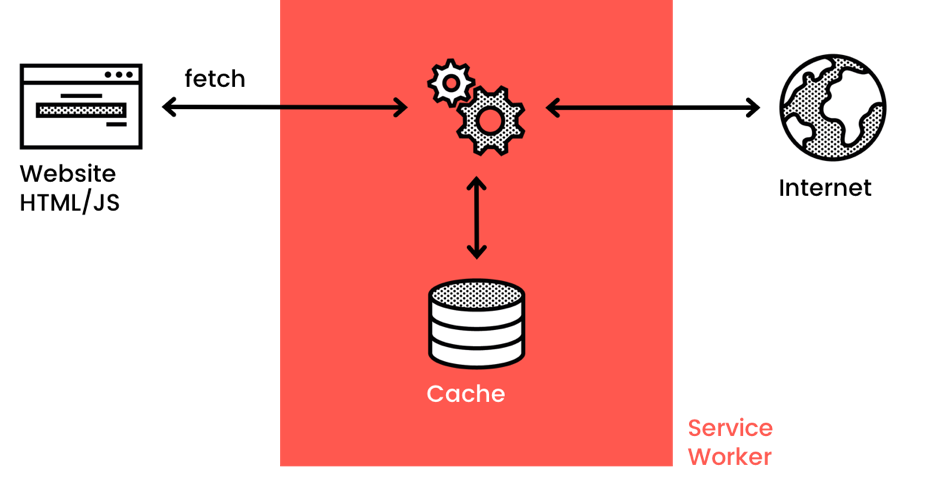
\includegraphics[width=1\linewidth]{src/ServiceWorker-Heise.png}
  \caption{Service Workers als Proxy\cite{src_serviceworker_heise}}
  \label{fig:heise_serviceworker}
\end{wrapfigure}

Folglich ist es also notwendig, einheitlich die Inhalte aus dem Netzwerk abzurufen, da sie dort immer erhältlich sind.
Werden diese Netzwerkanfragen dann noch lokal abgefangen, kann überprüft werden, ob ein Inhalt bereits lokal erhältlich ist.
Wenn dies der Fall ist, so ist es möglich, die Anfrage umzuleiten, sodass die lokalen Ressourcen verwendet werden.
Für die lokale Verwaltung von Inhalten sind die sogenannten \enquote{Service Worker} zuständig, dessen Funktionsweise im folgenden näher erläutert wird.

Wie andere Arten der \enquote{Worker} sind Service Worker auch ein JavaScript-Programm, das in einem eigenen Kontext läuft.
Dieser Kontext ermöglicht die Verwendung mehrerer Threads in JavaScript, da jeder Kontext in einem eigenen Thread laufen kann.
So ist ein Service Worker im Hintergrund aktiv und kann dort auf Events reagieren.
Dabei haben Service Worker jedoch keinen direkten Zugriff auf das \ac{dom} der \ac{pwa}.

In dem globalen Kontext der Service Worker befindet sich ein Cache-Objekt, welches den lokalen Speicher der \ac{pwa} repräsentiert\cite{w3c_serviceworker_nightly}.
Dieser Cache muss zunächst populiert werden, was entweder bei der Installation der \ac{pwa} oder zu späterem Zeitpunkt mit der ersten Anfrage einer Ressource geschehen kann\cite{ServiceWorker_explained}.
Anschließend kann bei Anfragen von gecachten Inhalten, auf den Cache verwiesen werden.

Das Reagieren auf Anfragen geschieht über ein \enquote{fetch}-Event, auf welches Service Worker reagieren können.
Für dieses Event kann eine Funktion registriert werden, welche ein Event-Objekt als Parameter akzeptiert.
Das Event-Objekt enthält alle Informationen über die angeforderte Ressource und kann manipuliert werden, um auszuwählen, von wo die Ressource geladen werden soll.
Wenn der Cache bereits populiert ist, ist die Auswahl über den Cache trivial.

\begin{figure}[h]
\begin{lstlisting}[language=java]
  self.addEventListener('fetch', function(event) {
    event.respondWith(caches.match(event.request)
      .then(cachedResponse => cachedResponse || fetch(event.request)))
  });
\end{lstlisting}
\caption{Auswahl von Ressourcen aus dem Cache.\cite{heise_pwa2}}
\label{fig:js_cache}
\end{figure}

Wie in Abbildung \ref{fig:js_cache} dargestellt, wird eine anonyme Funktion für das \enquote{fetch}-Event registriert.
Diese Funktion legt fest, dass auf die Anfrage des \enquote{fetch}-Event eine Antwort aus dem Cache gesucht werden soll.
Wenn die angeforderte Ressource im Cache vorhanden ist, wird sie als Ergebnis der Anfrage festgelegt.
Andernfalls wird eine Anfrage über das Netzwerk gesendet, um die Ressource abzurufen.

Durch die Funktionsweise von Service Workern stellen diese gleichzeitig ein großes Sicherheitsrisiko dar.
Wenn ein Dritter einen Service Worker zwischen Server und Nutzer manipulieren würde, hätte dieser Zugriff auf alle Netzwerkanfragen, die der Nutzer der \ac{pwa} sendet.
Um Angriffe eines solchen Mittelmannes zu verhindern, dürfen Service Worker laut Spezifikation nur über HTTPS ausgeliefert werden.
Dabei wird der Übertragungskanal verschlüsselt, wodurch eine Manipulation des Service Worker durch Dritte nicht möglich ist.

% TODO Gegenlesen: Ressource vs. Inhalt

Durch Service-Worker ist es also möglich, einen Cache in jede Website einzubinden.
Da diese im Hintergrund arbeiten und auf bereits vorhandene Technologien aufbauen, ist es nicht einmal nötig, eine bereits vorhandene Website anzupassen, um den Cache zu implementieren.


\subsection{Interaktion mit Nutzern}

Eine weiteres Merkmal von \acp{pwa}, welches herkömmliche Websites nicht besitzen, ist die Art und Weise, wie mit Nutzern interagiert wird.
Native Anwendungen können auf Ressourcen des Betriebsystems zugreifen, um mit dem Nutzer zu interagieren selbst wenn die Anwendung nicht aktiv vom Nutzer verwendet wird.
Weit verbreitet ist beispielsweise das Verwenden von Push-Notifications\cite{businessofapps_pushnotificationstatistics}, um Nachrichten oder Informationen an den Nutzer zu leiten.

\acp{pwa} sind ebenso in der Lage, Push-Notifications zu senden, was sie von herkömmlichen Websites abgrenzt.
Diese können auch Benachrichtigungen senden, jedoch nur, wenn der Nutzer aktiv eine Seite betrachtet.
Durch Service-Worker, welche unabhängig eines Seitenaufrufs ausgeführt werden, können \acp{pwa} auch Benachrichtigungen senden, ohne dass die \ac{pwa} geöffnet ist\cite{ejaz_progressive_pushnotifications}.

\begin{figure}[h]
  \centering
  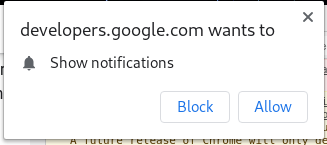
\includegraphics[width=0.4\linewidth]{src/permission-request-chrome.png}
  \caption{Google Chrome fragt um die Zustimmung des Nutzers.}
  \label{fig:chrome_permission}
\end{figure}

Zunächst muss ein Nutzer zustimmen, dass er Benachrichtigungen von einer Website oder \ac{pwa} erhalten will.
Falls die Zustimmung erteilt wird, wird dies für die entsprechende Website oder \ac{pwa} gespeichert, sodass eine Zustimmung nur ein einziges Mal eingeholt werden muss, so lange der Nutzer nicht im Nachhinein die Berechtigung widerruft.

Auf einer geöffneten Website genügt die Zustimmung des Nutzers, um eine Benachrichtigung anzuzeigen.
Der beim Seitenaufruf ausgeführte JavaScript-Code kann aktiv eine Benachrichtigung erstellen und anzeigen.
Eine \ac{pwa}, die nicht ausgeführt wird, kann auf diesen Weg keine Benachrichtigung anzeigen.
Auch der Service-Worker kann nicht aktiv eine Benachrichtigung erstellen, da dieser nur auf externe Events reagieren kann.

Folglich werden Push-Notifications nicht vom eigenen Gerät erstellt, sondern nur auf diesem angezeigt.
Für das Empfangen der Benachrichtigungen wird die Push-API\cite{w3c_pushapi} verwendet.
Über diese API kann sich ein Service-Worker bei dem Push-Client des Browsers registrieren, welcher mit einem Push-Service zusammenarbeitet.



Für das Senden einer Push-Notification wird nun von einem Backend aus eine Anfrage über das \textit{Web Push Protocol}\cite{ietf_webpush} an den Push-Service gesendet.
Dieser Verteilt dann die Push-Notification an alle registrierten Clients, die die Benachrichtigung erhalten sollen.
Falls ein Client offline ist, wird die Benachrichtigung in eine Warteschlange eingefügt und zugestellt, wenn der Client eine erneute Verbindung aufbaut\cite{googledev_webpush}.

\begin{figure}[h]
  \centering
  
\includegraphics[width=\textwidth]{src/Push-API.png}
  \caption{Ablauf beim Senden einer Push-Notification}
  \label{fig:push_api}
\end{figure}


Der Client leitet dann die erhaltene Push-Notification als Event an den entsprechenden Service-Worker weiter, welcher so auf die Benachrichtigung reagieren kann.
So ist es für den Service-Worker nun möglich, eine native Benachrichtigung auf dem Gerät des Nutzers anzuzeigen und das, obwohl die \ac{pwa} des Service-Workers nicht aktiv ist, da dieser unabhängig zur \ac{pwa} ausgeführt wird.


\subsection{Interaktion mit Systemressourcen}

Um mit nativen Anwendungen mithalten zu können, benötigen \acp{pwa} auch Zugriff auf die sonst geschützten Systemressourcen.
Für native Anwendungen ist der Zugriff auf Systemressourcen wie das Dateisystem oder angeschlossene Geräte meist keine große Hürde.
Falls überhaupt, muss vor Zugriff die Erlaubnis des Nutzers eingeholt werden, wofür native Schnittstellen vorliegen.
Damit auch Webanwendungen und somit \acp{pwa} auf diese Ressourcen zugreifen können, wird die Unterstützung des Browsers benötigt, welcher als Schnittstelle zwischen Webanwendung und den nativen Ressourcen agiert.

Es ergibt sich dadurch jedoch die Herausforderung, eine einheitliche Schnittstelle zu schaffen, sodass eine Webanwendung unabhängig vom Browser auf Systemressourcen zugreifen kann.
Darauf folgt, dass für jede Zugriffskomponente ein eigener Standard entwickelt wird, welcher anschließend in den einzelnen Browsern umgesetzt werden muss.

Zum aktuellen Zeitpunkt existieren für nahezu alle Zugriffskomponenten, die ein Smartphone oder PC bietet, ein Standard oder zumindest ein Entwurf für diesen.
In einer Übersicht von Adam Bar\cite{bar_webcando} werden insgesamt 44 dieser Komponenten gelistet.
Als Folge dieser großen Vielfalt ist eine ebenso große Vielfalt an Zugriffsformen, die in den Standards festgelegt sind.

\paragraph{Positionsdaten} Positionsdaten werden über ein \textit{Geolocation}-Objekt im Navigator des Browsers angefordert.
Eine Überprüfung, ob dieses Objekt vorhanden ist, genügt, um Kompatibilität des Browsers festzustellen.
Beim Anfragen der Positionsdaten wird dann automatisch um Erlaubnis des Nutzers gebeten\cite{w3c_geolocation}.

\paragraph{Benachrichtigungen} Benachrichtigungen können über ein \textit{Notification}-Objekt erstellt werden. Dieses befindet sich im globalen Kontext eines Tabs.
Bevor eine Benachrichtigung angezeigt werden kann, muss aktiv um Erlaubnis gebeten werden\cite{whatwg_notification}.

\paragraph{Kamera und Mikrophon} Geräte wie Kameras oder Mikrophone liefern einen dauerhaften Strom an Daten.
Diese Datenströme können über ein \textit{Media Devices}-Objekt im Navigator des Browsers angefordert werden\cite{w3c_mediacapture}.

Neben der großen Vielfalt an standardisierten Zugriffsformen unterscheidet sich auch, wie verbreitet die Implementierung der Standards ist.
Während der Zugriff auf Mikrophon und Kamera beispielsweise noch bei 95\% der Nutzer unterstützt ist, so ist das Erstellen und Anzeigen nur noch bei 77\% der Nutzer möglich\cite{caniuse}.
Hinzu kommt, dass die Implementierungen in den verschiedenen Browsern fehlerhaft sind, sodass je nach Browser des Benutzers, Fehler innerhalb der Webanwendung auftauchen können.

Trotz der großen Vielfalt gibt es auch einige Komponenten, auf welche \acp{pwa} keinen Zugriff haben.
Ein Zugriff auf Telefonie-Funktionen existiert nicht.
\acp{pwa} können also keine Anrufe starten oder SMS schreiben und empfangen.
Ebenso bleibt der Zugriff auf spezialisierte Geräte verwehrt, da es keinen einheitliche Form für den Zugriff gibt.
Zu den Geräten, die nicht angesteuert werden können, zählt beispielsweise die Taschenlampe eines Smartphones.

Allgemein betrachtet ist zu sagen, dass bereits auf viele Systemressourcen zugegriffen werden kann, wodurch \acp{pwa} viele Funktionen nativer Anwendungen übernehmen können.
Jedoch bleibt zu beachten, dass für den Zugriff auf diese Ressourcen jeweils der Browser auch die entsprechenden Berechtigungen benötigt.

Zu beachten ist jedoch, dass der Browser als Schnittstelle zwischen Webanwendung und System ein eigenes System der Rechteverwaltung implementieren muss, damit nicht jede Webanwendung automatisch auf die selben Ressourcen zugreifen kann, für die dem Browser der Zugriff gestattet ist.

% TODO pwa vs Webanwendung

\subsection{Browserspezifische Voraussetzungen}

Nachdem nun besprochen wurde, welche Voraussetzungen nötig sind, um das Funktionieren einer \ac{pwa} zu gewährleisten, werden nun die Voraussetzungen aufgezählt, die die einzelnen Browser an eine Webanwendung stellen, um diese dem Nutzer als \ac{pwa} vorzustellen.

Hierbei wird ein besonderer Schwerpunkt auf die Browser \textit{Google Chrome}, \textit{Mozilla Firefox} und \textit{Microsoft Edge} gelegt.
In deren Dokumentation\cite{googledev_pwainstallcriteria,docsmicrosoft_pwainstallcriteria,mozilladev_pwainstallcriteria} existiert ein Abschnitt \enquote{\ac{aths}}, welcher sich mit dem Installationsvorgang einer \ac{pwa} befasst.
\ac{aths} beschreibt die Installation einer \ac{pwa}, wobei dem Nutzer zunächst ein Installationsdialog gezeigt wird, dessen Bestätigung die \ac{pwa} lokal verfügbar macht und eine Verknüpfung zur jener auf dem Home Screen des Nutzers erstellt.


\paragraph{Google Chrome}
Damit der Google Chrome Browser einen Installationsdialog zum Installieren einer \ac{pwa} anzeigt, ist zunächst einmal die wichtigste Voraussetzung, dass die aktuell betrachtete Webanwendung nicht bereits installiert ist.
Dadurch soll sichergestellt werden, dass in erster Linie die Notwendigkeit besteht, die \ac{pwa} zu installieren.
Dazu zählt des Weiteren, dass der Nutzer eine heuristische Erwartung erfüllt, die Anwendung zu installieren.
Wird aus der Interaktion eines Nutzers mit einer Webanwendung nicht erkenntlich, dass er bereit wäre, diese zu installieren, so wird kein Dialog angezeigt.
Zu dieser Heuristik äußert sich Google nicht weiter, gibt aber bekannt, dass in einer früheren Version eine \enquote{30 sekündige Interaktion mit der Domain} notwendig gewesen war.
Ist also erkennbar, dass ein Nutzer Installationsabsichten besitzt, werden die Kriterien der \ac{pwa} geprüft.
Die \ac{pwa} muss einen Service-Worker registriert haben und über HTTPS an den Nutzer ausgeliefert werden, um für eine Installation in Frage zu kommen.
Zudem muss eine Manifestdatei bestehen, welche mindestens den Namen der \ac{pwa}, eine Start-URL und Icons in der Größe $192\times192$ sowie $512\times512$ Pixel definiert.

\paragraph{Mozilla Firefox}
Die Kriterien des Firefox Browsers sind weniger streng als die von Google Chrome.
Hier wird auch verlangt, dass eine \ac{pwa} über HTTPS an den Nutzer ausgeliefert wird und dass sie eine Manifestdatei enthält.
Eine bestimmte Interaktion des Nutzers mit der \ac{pwa} wird nicht verlangt.
Die Manifestdatei muss ähnlich wie bei Google Chrome den Namen der \ac{pwa}, eine Start-URL und passende Icons definieren.
Zudem wird noch eine Hintergrundfarbe verlangt.

\paragraph{Microsoft Edge}
Der Edge Browser stellt ähnliche Anforderungen an eine \ac{pwa} wie die bisher besprochen Browser.
Es wird erwartet, dass die \ac{pwa} über HTTPS an den Nutzer ausgeliefert wird und Service Worker registriert hat.
Ebenso wird eine Manifestdatei verlangt, jedoch nicht angegeben, welche Felder diese mindestens definieren muss.
Da der Unterpunkt \enquote{Web app manifest} in der Dokumentation des Edge Browsers auf die von Mozilla verweist, ist anzunehmen, dass die Anforderungen an die Manifestdatei denen der anderen Browser entsprechen.

\paragraph{Weiter Browser}
Weitere Browser wie Opera\cite{devopera_pwainstallcriteria}, Samsung Internet\cite{samsung_pwainstallcriteria} oder der UC Browser\cite{ucweb_pwainstallcriteria} definieren ähnliche Kriterien für die Installation einer \ac{pwa}.
Sowohl das Ausliefern einer \ac{pwa} über HTTPS als auch das Vorhandensein von Service Workern zieht sich als roter Faden durch die Kriterien.
Des Weiteren wird von jedem Browser die Manifestdatei der \ac{pwa} verlangt.

Die Voraussetzungen der verschiedenen Browser sind größtenteils identisch.
Es ist festzustellen, dass die Voraussetzungen größtenteils das abdecken, was zum installieren einer \ac{pwa} notwendig ist.
Service Worker sind notwendig, um die \ac{pwa} lokal verfügbar zu machen.
Ohne HTTPS können Service Worker nicht verwendet werden.
Dadurch sind die meisten Voraussetzungen der Browser bereits abgedeckt.
Des Weiteren wird die Manifestdatei vorausgesetzt, welche definiert, wie die \ac{pwa} installiert wird.
Weitere Voraussetzungen sind nicht nötig, um die Anwendung installieren zu können.
Die von Google Chrome definierte Voraussetzung, dass ein Nutzer zunächst mit einer Domain interagieren muss, soll lediglich das Nutzererlebnis verbessern.


\section{Vorteile von \acp{pwa}}

\acp{pwa} bringen einige Vorteile mit sich.
Nutzern wird durch \acp{pwa} ein natives Nutzererlebnis für häufig genutzte Webanwendungen geboten.
Zudem verbrauchen \acp{pwa} zumeist deutlich weniger Speicher als eine native Anwendung, da nur die Manifestdatei, ein Icon und einige lokale Dateien gespeichert werden.
Gerade für Nutzer von Mobilgeräten ist dies von Vorteil, da solche Geräte wenig Ressourcen bieten, die durch \acp{pwa} weniger belastet werden.

Die größten Vorteile entstehen jedoch aus Sicht der Entwickler und Anbieter einer \ac{pwa}.
Durch Service Worker und Manifestdateien ist es möglich, eine bereits bestehende Webanwendung ohne großen Extraaufwand zu einer \ac{pwa} zu erweitern.
Die Entwicklungskosten sind im Vergleich zu einer nativen Anwendung deutlich geringer.
Zudem bieten \acp{pwa} bessere Möglichkeiten zur Interaktion mit dem Nutzer.
Aufgrund der URL-basierten Grundlage einer \ac{pwa}, ist es für Nutzer sehr einfach, Inhalte zu teilen, wodurch sich eine \ac{pwa} deutlich schneller als eine native Anwendung verbreiten kann.
Durch Push-Benachrichtigungen können Nutzer dann zu weiterer Interaktion mit der Anwendung animiert werden.
Es ist also zu erwarten, dass eine \ac{pwa} mehr Nutzer erhält als eine herkömmliche Webanwendung oder eine native App.
Ein weiterer Vorteil für Entwickler ist, dass Aktualisierungen sofort bei Nutzung der \ac{pwa} installiert werden können.
Die Service Worker ermöglichen es, immer die aktuellsten Dateien herunterzuladen, ohne dass der Nutzer manuell eine Aktualisierung durchführen muss.
So können neue Features leichter durchgesetzt werden und die gezwungene Unterstützung für ältere Versionen entfällt.

Die meisten Vorteile von \acp{pwa} entstehen also für Entwickler und Anbieter, welchen schnellere und günstigere Entwicklung ermöglicht wird.
Zusammen mit einer höheren Nutzerinteraktion und Motivation kann sich eine \ac{pwa} so durchaus als lukrativ erweisen.
Für Nutzer bieten \acp{pwa} ein natives Nutzererlebnis und die Möglichkeit, ressourcenschonende Anwendungen zu nutzen.


\section{Kritik an \acp{pwa}}

Die größten Kritikpunkte an \acp{pwa} entstehen durch die Kerneigenschaften dieser.
Als Webanwendungen müssen sie von einem Browser ausgeführt werden, welcher zumeist eine hochkomplexe Anwendung ist.
Dies ist gerade auf Mobilgeräten ein Problem, welche durch eine Batterie nur begrenzte Spannungsversorgung haben.
Das Ausführen des Browsers zusammen mit der eigentlichen Anwendung erhöht den Batterieverbrauch, wodurch gerade Nutzer auf schwächeren Geräten davon absehen werden, die \ac{pwa} zu verwenden.
Ein weiteres Problem ist der Zugriff auf Systemressourcen und Geräte durch den Browser.
\acp{pwa} können längst nicht alle Aktivitäten ausführen, zu denen native Anwendungen in Stande sind.
Des weiteren entsteht die Problematik, dass verschiedene Browser verschiedene Schnittstellen für \acp{pwa} bieten.
Es kann also nicht garantiert werden, dass eine \ac{pwa} für jeden Nutzer funktioniert.
Gerade bei iOS-Geräte wird dies zu einem Problem, da auf dieser Plattform die Unterstützung für \acp{pwa} erst spät eingeführt wurde.

Ein weiterer Aspekt, der kritisch beachtet werden muss, ist die Sicherheit von \acp{pwa}.
Im Vergleich zu nativen Anwendungen gibt es nämlich keine einheitliche Instanz, die für den Vertrieb und die Kontrolle der Anwendungen zuständig ist.
So muss dem Anbieter der \ac{pwa} vertraut werden, dass diese sowohl sicher als auch frei von eventueller Schadsoftware ist.
Die Möglichkeit, mit einer \ac{pwa} Schadsoftware zu installieren, ist besonders in Hinsicht auf Service Worker bedenklich, welche den Kern einer \ac{pwa} ausmachen.
Deren Position ermöglicht es, alle von einer Anwendung gestellten Netzwerkanfragen zu unterbinden und umzuleiten.

Die größten Kritikpunkte liegen also im Bereich der Sicherheit, das \acp{pwa} ohne weitere Kontrolle installiert werden können.
Jedoch ist auch zu bedenken, dass der Funktionsumfang einer \ac{pwa} immer an den Browser eines Nutzers angepasst werden muss, was zur Folge hat, dass manche Nutzer die Webanwendung nur eingeschränkt oder gar überhaupt nicht verwenden können.

\newpage

\section{Fazit}
\label{sec:fazit}

Als Fazit ergibt sich, dass \acp{pwa} weder herkömmliche Webanwendungen noch native Anwendungen vollständig ersetzen können.
Mit dem Anspruch, die Lücke zwischen diesen beiden Kategorien von Anwendungen zu füllen, verbinden \acp{pwa} zwar viele gute Eigenschaften beider Welten, können jedoch noch nicht alle Einsatzgebiete übernehmen.

Für Nutzer bieten \acp{pwa} eine nahezu nahtlose Integration in die bereits bestehenden Strukturen nativer Apps und bestechen zudem mit geringerem Speicherverbrauch und schnelleren Ladezeiten.
Viel mehr ist aber aus Nutzersicht nicht geboten.
Hinzu kommt, dass \acp{pwa} keine Eigenständigen Anwendungen sind und daher immer die Unterstützung des Browsers benötigen, welcher viele Ressourcen benötigt, was sich besonders im Akkuverbrauch auf Mobilgeräten kenntlich macht.

Für Entwickler haben \acp{pwa} mehr zu bieten.
Eine einfache Migration von existierenden Webanwendungen, sofortige Aktualisierungen für die gesamte Nutzerbasis und ein breiter Zugriff auf Systemressourcen, eröffnen für Webanwendungen völlig neue Gebiete und ermöglicht eine schnellere Softwareentwicklung, wodurch Entwicklungskosten sinken.
Für Entwickler bleibt dabei jedoch zu beachten, dass die Unterstützung für \acp{pwa} browserspezifisch ist, was die Testkosten erhöhen kann oder im schlimmsten Fall, die Nutzung der \ac{pwa} einschränkt.

Voraussichtlich werden sich \acp{pwa} in Bereichen durchsetzen, wo ein großteil der Inhalte in Echtzeit aus dem Internet stammt.
Sozial Media, Online Zeitschriften und Videoplattformen werden wohl am meisten von den \acp{pwa} profitieren.
Anstelle viele native Anwendungen zusätzlich zu der bereits existierenden Webanwendung zu entwickeln, kann diese zu einer \ac{pwa} weiterentwickelt werden und so eine große Anzahl an Nutzern erreichen.
Für Seiten mit statischen Inhalten wird es kaum lohnenswert sein, in den zusätzlichen Entwicklungsaufwand für eine \ac{pwa} zu investieren.
Ebenso werden native Anwendungen nicht verdrängt werden, da der direkte Systemzugriff für einige Bereiche notwendig ist, sodass beispielsweise Telefonie nicht aus einer Webanwendung heraus möglich ist.

Wie stark sich \acp{pwa} tatsächlich durchsetzen werden, wird lediglich die Zeit zeigen können, mit welcher \acp{pwa} wohl zunehmend an Unterstützung gewinnen werden.
Welche Konsequenzen sich daraus ergeben werden, sollte ein Großteil unserer Anwendungen tatsächlich von verteilten Anbietern aus dem Internet kommen statt einer zentralen Stelle, wie es bisher der Trend war, ist auch noch nicht abzusehen.

\newpage

\spacing{1}

\printbibliography

\end{document}

%%% Local Variables:
%%% mode: latex
%%% TeX-master: t
%%% End:
